\section{Teorema de Green}
\begin{definición}[Curva de Jordan]
Una curva de Jordan $C$ en $\mathbb{R}^2$ es la imagen de un camino cerrado y simple en $\mathbb{R}^2$, es decir, $C = Im(\gamma)$ con $\gamma: [a,b] \to \mathbb{R}^2$ continua, inyectiva en $[a, b)$ y $\gamma(a) = \gamma(b)$.
\end{definición}
Dicho de otra forma, una curva de Jordan en el plano es una curva cerrada y continua que no se cruza a sí misma. Es como si tomaras un lápiz, dibujaras una línea continua sin levantarlo del papel, sin pasar dos veces por el mismo punto (excepto al final), y al final volvieras exactamente al punto de partida.

Más técnicamente, es la imagen de una función continua \( \gamma \) que recorre
la curva desde un punto inicial \( \gamma(a) \) hasta un punto final \(
\gamma(b) \), con la condición de que todos los puntos intermedios son
distintos (no hay autointersecciones), y solo el inicio y el final coinciden:
\( \gamma(a) = \gamma(b) \). Este tipo de curva encierra una región bien
definida del plano, como un lazo o un contorno cerrado limpio.\\

\begin{observación}
Se puede demostrar que $C$ es un homeomorfa a la circunferencia unitaria $S^1$.
\end{observación}
\begin{teorema}[Teorema de la curva de Jordan]
    Toda curva de Jordan $C$ en $\mathbb{R}^2$ divide al plano en dos regiones  o componentes conexas, una acotada, denominada \underline{parte interior a $C$} y otra no acotada, denominada \underline{parte exterior a $C$}, siendo $C$ la frontera común a ambas regiones. Es decir,
    $$\mathbb{R}^2 = Int(C) \cup Ext(C) \cup C \text{ con } \begin{cases}
            Int(C) = \text{abierto conexo acotado} \\ Ext(C) = \text{ abierto conexo no acotado} \\ Fr(Int(C)) = C = Fr(Ext(C))
        \end{cases} \text{ unión disjunta}$$
\end{teorema}
\begin{definición}[Conexión Simple]
Un conjunto abierto y conexo $U \subset \mathbb{R}^2$ se dice que es simplemente conexo si $\forall C$ curva de Jordan en $U$ se tiene que $Int(C) \subset U$.
\end{definición}

Informalmente, podemos definir un conjunto simplemente conexo como aquel que no
tiene agujeros, es decir, toda curva de Jordan que esté dentro del conjunto
también encierra completamente una región que pertenece al conjunto. Por
ejemplo, el disco abierto \( D = \{(x, y) \in \mathbb{R}^2 : x^2 + y^2 < 1\} \)
es simplemente conexo, mientras que el conjunto \( \mathbb{R}^2 \setminus
\{(0,0)\} \) no lo es, porque tiene un agujero en el origen.\\

\begin{definición}[Orientación de una Curva de Jordan]
Sea $C \subset \R^2$ curva de Jordan de clase $C^1$ a trozos. Se define la orientación positiva en $C$ y se denota $C^+$ como el sentido de recorrido contrario a las agujas del reloj. \\
Conceptualmente, es el sentido de recorrido que deja la parte interior de $C$ a la izquierda.
\end{definición}

\begin{teorema}[Teorema de Green]
    Sean $C$ curva de Jordan regular a trozos con parte interior $D = Int(C)$, $\vec{F} = (P, Q) : U \to \R^2$ campo vectorial de clase $C^1$ definido en un abierto $U \supset \overline{D} = D \cup C$. Entonces:
    $$\int_{C^+} P \, dx + Q \, dy = \int_{D} \left(\frac{\partial Q}{\partial x} - \frac{\partial P}{\partial y}\right) dx \, dy
    $$
    donde $C^+$ representa la curva $C$ con orientación positiva.
\end{teorema}

\begin{proof}
    Para el caso de dominios que son a la vez proyectables horizontalmente y verticalmente. Es decir, supongamos que
    $$\overline{D} = \left\{ (x,y) \in \R^2 \mid a \leq x \leq b, \ f(x) \leq y \leq g(x) \right\}$$
    donde las funciones $f,g: [a,b] \to \R$ son de clase $C^1$.\\
    Entonces $C^+ = \gamma_1 + \gamma_2 - \gamma_3 - \gamma_4$ donde
    $$\begin{cases}
            \gamma_1(t) = (t, f(t)), \quad t \in [a,b] \quad \gamma_1'(t) = (1, f'(t)) \neq (0,0) \\
            \gamma_2(t) = (b,t) \quad t \in [c_2, d_2] \quad \gamma_2'(t) = (0,1)                 \\
            \gamma_3(t) = (t, g(t)) \quad t \in [a,b] \quad \gamma_3'(t) = (1, g'(t)) \neq (0,0)  \\
            \gamma_4(t) = (a,t) \quad t \in [c_4, d_4] \quad \gamma_4'(t) = (0,1)
        \end{cases}$$

    Entonces,

    \begin{itemize}
        \item
              \[
                  \int_{C^+} Pdx + Qdy = \int_{C^+} Pdx + \int_{C^+} Qdy
                  \implies \int_{C^+} Pdx = \int_{\gamma_1+\gamma_2-\gamma_3-\gamma_4} (P,0)
              \]
              \[
                  = \int_{t=a}^{t=b} \left\langle (P(t,f(t)), 0), (1, f'(t)) \right\rangle dt
                  + \int_{t=c_2}^{t=d_2} \left\langle (P(b,t), 0), (0,1) \right\rangle dt
              \]
              \[
                  - \int_{t=a}^{t=b} \left\langle (P(t,g(t)), 0), (1, g'(t)) \right\rangle dt
                  - \int_{t=c_4} ^{t=d_4} \left\langle (P(a,t), 0), (0,1) \right\rangle dt
              \]
              \[
                  = \int_{t=a}^{t=b} P(t,f(t)) - P(t,g(t)) dt
              \]

        \item
              \[
                  \int_{D} -\frac{\partial P}{\partial y}dxdy
                  = -\int_{x=a}^{x=b} \int_{y=f(x)}^{y=g(x)} \frac{\partial P(x,y)}{\partial y} dy \,dx
                  = -\int_{x=a}^{x=b} \left[ P(x,y) \right] _{y=f(x)}^{y=g(x)} dx
              \]
              \[
                  = -\int_{x=a}^{x=b} P(x,g(x)) - P(x,f(x)) dx
                  = \int_{x=a}^{x=b} P(x,f(x)) - P(x,g(x)) dx
              \]
    \end{itemize}

    Usando que $\overline{D}$ es verticalmente proyectable, hemos obtenido que
    $\int_{C^+} Pdx = -\int_{D} \frac{\partial P}{\partial y}dxdy$.\\ Usando que
    $\overline{D}$ es horizontalmente proyectable, veamos que $\int_{C^+} Qdy =
        \int_{D} \frac{\partial Q}{\partial x}dxdy$.\\ Suponemos entonces que
    $$\overline{D} = \left\{ (x,y) \in \R^2 \mid c \leq y \leq d, \ \varphi(y) \leq
        x \leq \psi(y) \right\}$$ donde $\varphi, \psi: [c,d] \to \R$ son de clase
    $C^1$.\\ Entonces $C^+ = \sigma_1 - \sigma_2 - \sigma_3 + \sigma_4$ donde $$
        \begin{cases}
            \sigma_1(t) = (\psi(t), t), \quad t \in [c,d] \quad \sigma_1'(t) = (\psi'(t), 1)       \\
            \sigma_2(t) = (t, d), \quad t \in [a_2, b_2] \quad \sigma_2'(t) = (1, 0)               \\
            \sigma_3(t) = (\varphi(t), t), \quad t \in [c,d] \quad \sigma_3'(t) = (\varphi'(t), 1) \\
            \sigma_4(t) = (t, c), \quad t \in [a_4, b_4] \quad \sigma_4'(t) = (1, 0)
        \end{cases}
    $$

    \begin{itemize}
        \item $$\int_{C^+} Qdy = \int_{\sigma_1 - \sigma_2 - \sigma_3 + \sigma_4} (0,Q) $$
              $$= \int_{t=c}^{t=d} \langle (0,Q(\psi(t),t)), (\psi'(t),1) \rangle dt - \int_{t=a_2}^{t=b_2} \langle (0,Q(t,d)), (1,0) \rangle dt $$
              $$- \int_{t=c}^{t=d} \langle (0,Q(\varphi(t),t)), (\varphi'(t),1) \rangle dt + \int_{t=a_4}^{t=b_4} \langle (0,Q(t,c)), (1,0) \rangle dt $$
              $$= \int_{t=c}^{t=d} Q(\psi(t),t) - Q(\varphi(t),t) dt$$
        \item $$\int_{D} \frac{\partial Q}{\partial x}dxdy = \int_{y=c}^{y=d} \int_{x=\varphi(y)}^{x=\psi(y)} \left( \frac{\partial Q(x,y)}{\partial x} dx \right) dy = \int_{y=c}^{y=d} Q(\psi(y),y) - Q(\varphi(y),y) dy$$
    \end{itemize}

\end{proof}

El Teorema de Green establece una conexión profunda entre una integral de línea
alrededor de una curva cerrada y una integral doble sobre la región encerrada
por esa curva. En esencia, dice que recorrer el campo vectorial a lo largo del
borde de una región (lado izquierdo) es equivalente a acumular la rotación o
“vorticidad” del campo dentro de esa región (lado derecho).

En términos geométricos, si tienes un campo vectorial \(\vec{F} = (P, Q)\), el
teorema afirma que el trabajo total que realiza ese campo al recorrer la curva
cerrada \(C^+\) (es decir, la integral de línea) es igual a la suma de las
diferencias entre los cambios de \(Q\) en \(x\) y de \(P\) en \(y\) en el
interior de la curva (es decir, una integral de área del rotacional escalar).
El teorema es válido siempre que el campo sea suficientemente suave y que la
región encerrada no tenga agujeros.\\

\begin{observación}
$$\int_{D} \left(\frac{\partial Q}{\partial x} - \frac{\partial P}{\partial y}\right)dxdy = \int_{\overline{D}} \left(\frac{\partial Q}{\partial x} - \frac{\partial P}{\partial y}\right)dxdy$$
puesto que $C$ tiene área $D$.
\end{observación}

\begin{corolario}
    Sea \( C \subset \mathbb{R}^2 \) una curva de Jordan regular a trozos con parte interior \( D = \text{Int}(C) \), entonces se tiene que:
    \[
        \text{área}(D) = \int_{C^+} x\, dy = -\int_{C^+} y\, dx = \int_{C^+} \frac{1}{2} \left( x\, dy - y\, dx \right)
    \]
\end{corolario}

\begin{proof}

\end{proof}

\ejemplo{
    Vamos a verificar el Teorema de Green para el campo $\vec{F} = (x^2, xy)$ y la curva de Jordan $C$ dada por el borde del cuadrado $[0,1]^2$.\\
    $$
        \begin{cases}
            P(x,y) = x^2 \\
            Q(x,y) = xy
        \end{cases}
    $$

    $$
        \begin{cases}
            \gamma_1(t) =(t,0), \quad t \in [0,1] \quad \gamma_1'(t) = (1,0) \\
            \gamma_2(t) =(1,t), \quad t \in [0,1] \quad \gamma_2'(t) = (0,1) \\
            \gamma_3(t) =(t,1), \quad t \in [0,1] \quad \gamma_3'(t) = (1,0) \\
            \gamma_4(t) =(0,t), \quad t \in [0,1] \quad \gamma_4'(t) = (0,1) \\
        \end{cases}
    $$

    \begin{itemize}
        \item $$\int_{C^+} x^2 dx + xy dy = \int_{\gamma_1 + \gamma_2 + \gamma_3 + \gamma_4} x^2 dx + xy dy$$
              $$= \underbrace{\int_{t=0}^{t=1} \langle (t^2, 0), (1,0) \rangle dt}_{\gamma_1} + \underbrace{\int_{t=0}^{t=1} \langle (1,t), (0,1) \rangle dt}_{\gamma_2} - \underbrace{\int_{t=0}^{t=1} \langle (t^2,t), (1,0) \rangle dt}_{\gamma_3} - \underbrace{\int_{t=0}^{t=1} \langle (0,0), (0,1) \rangle dt}_{\gamma_4}$$
              $$= \int_{t=0}^{t=1} t^2 dt + \int_{t=0}^{t=1} t dt - \int_{t=0}^{t=1} t^2 dt - 0 = \left[ \frac{t^2}{2} \right]_{t=0}^{t=1} = \frac{1}{2}$$
        \item $$\int_{D} \left( \frac{\partial Q}{\partial x} - \frac{\partial P}{\partial y} \right) dx dy = \int_{D} (y-0)dxdy = \int_{x=0}^{x=1} \left( \int_{y=0}^{y=1}ydy \right)dx = \left[ \frac{y^2}{2}\right] _{y=0}^{y=1} = \frac{1}{2}$$
    \end{itemize}

}

\ejemplo{

    Verificar el teorema de Green para la circunferencia de radio 2 y centro en el
    origen, el campo $\vec{F} = (x-y, x+y)$ .\\ $$
        \begin{cases}
            \gamma(t) = (2\cos(t), 2\sin(t)), \quad t \in [0,2\pi] \quad \gamma(0) = \gamma(2\pi) \text{ para } \gamma(0) \neq \gamma(t) \ \forall t \in (0,2\pi) \\
            \gamma'(t) = (-2\sin(t), 2\cos(t)) \neq (0,0)
        \end{cases}
    $$

    $$\overline{D} = \left\{ (x,y) \mid x^2+y^2 \leq 4 \right\}$$

    \begin{itemize}
        \item $$\int_{C^+} (x-y)dx + (x+y)dy = \int_{t=0}^{t=2\pi} \langle (2\cos(t) - 2\sin(t), 2\cos(t) + 2\sin(t)), (-2\sin(t), 2\cos(t)) \rangle dt $$
              $$= \int_{t=0}^{t=2\pi} (-4\cos(t)\sin(t) + 4\sin^2(t) + 4\cos^2(t) -4\sin(t)\cos(t))dt = \int_{t=0}^{t=2\pi} 4 dt = 8\pi$$
        \item $$\int_{\overline{D}} (1+1) dx dy = 2(\text{área}(\overline{D})) = 2 (\pi 2^2) = 8\pi$$
    \end{itemize}

}

\ejemplo{
    Sea el campo vectorial $F(x, y) = (x^2 +y^2, -3xy + xy^3 + y^2)$ sobre la curva definida por el cuadrado $[0, 1]^2$.
    Veamos dos maneras de calcular la integral de camino dada por $\int_{\gamma} F \cdot dr$.
    \begin{enumerate}
        \item Podemos describir la curva como producto de una concatenación de curvas:
              $\gamma = \gamma _1 \times \gamma _2 \times \gamma _3 \times \gamma _4$ donde:
              $$\begin{cases}
                      \gamma_1 \equiv (4t, 0) :  t \in [0, \frac{1}{4})              \\
                      \gamma_2 \equiv (1, 4t - 1) : t \in [\frac{1}{4}, \frac{2}{4}) \\
                      \gamma_3 \equiv (3 - 4t, 1) : t \in [\frac{2}{4}, \frac{3}{4}) \\
                      \gamma_4 \equiv (0, 4 - 4t) : t \in [\frac{3}{4}, 1]
                  \end{cases} \implies$$
              $$\int_{\gamma} F = \sum_{k = 1}^{4} \int_{t=\frac{k-1}{4}}^{t=\frac{k}{4}} \langle F(\gamma_k(t)), \gamma_k'(t) \rangle dt = \sum_{k = 1}^{4} \int_{t=\frac{k-1}{4}}^{t=\frac{k}{4}} \langle F(\gamma_k(t)), \gamma_k'(t) \rangle dt = $$

              $$
                  = \int_{t=0}^{t=\frac{1}{4}} \langle (4t)^2 + 0, -3 \cdot (4t) \cdot 0 + 4t \cdot 0^3 + 0 \rangle, (4,0) \rangle dt +
              $$

              $$
                  + \int_{t=\frac{1}{4}}^{t=\frac{2}{4}} \langle (t^2 + (4t-1)^2, -3(4t-1) + (4t-1)^3 + (4t-1)^2) \rangle, (0,4) \rangle dt +
              $$

              $$
                  + \int_{t=\frac{2}{4}}^{t=\frac{3}{4}} \langle (3-4t)^2 - 1^2, -3(3-4t) + (3-4t) + 1) \rangle, (-4,0) \rangle dt +
              $$

              $$
                  + \int_{t=\frac{3}{4}}^{t=1} \langle (4-4t)^2, (4-4t)^2 \rangle, (0,-4) \rangle dt
              $$
              Y resolveriamos las integrales polinómicas de forma usual.
        \item Otra forma de resolverlo es aplicando el teorema de Green: \\ Para ello veamos
              que el camino definido anteriormente sea una Curva de Jordan $$\begin{cases}
                      \text{Simple: } \forall t_1, t_2 \in (a,b) : t1 \neq t_2 \implies \gamma(t_1) \neq \gamma(t_2) \\
                      \text{Cerrada: } \gamma(0) = \gamma(1)                                                         \\
                      \text{Regular: } ||\gamma'(t)|| \neq 0 \ \forall t \in [0,1]
                  \end{cases} \implies \text{ es una curva de Jordan}$$
              Entonces tenemos que:
              $$\frac{\partial Q}{\partial x} =   -3y + y^3 \quad \frac{\partial P}{\partial y} = 3y^2 \implies$$
              $$\int_{\gamma} F = \int_{y=0}^{y=1} \left(\int_{x=0}^{x=1} -3y^2 +y^3 -3y^2 dx \right)dy = \int_{y=0}^{y=1} \left( \int_{x=0}^{x=1} -3y^2 + y^3 - 3y^2 \, dx \right) dy$$
              $$= \int_{x=0}^{x=1} -3y^2 + y^3 - 3y^2 \, dx = \left[\frac{-3y^2}{2} + \frac{y^4}{4} + \frac{-3y^3}{3}\right]^{x=1}_{x=0} = -\frac{3}{2} + \frac{1}{4} - 1 = -\frac{9}{4}$$
    \end{enumerate}
}

\ejemplo{
    Sea el campo vectorial $F(x,y) = \left(\frac{-y}{x^2 + y^2}, \frac{x}{x^2 + y^2}\right)$ y el camino dado por:
    $$\begin{cases}
            \gamma(t) = (8 + 3\cos(2\pi t), 6 +3\sin(2\pi t)) \\
            \gamma'(t) = 6\pi\left(-\sin(2\pi t), \cos(2\pi t)\right)
        \end{cases} \qquad t \in [0,1]
    $$
    Veamos cómo lo haríamos a través de la definición:
    $$\int_{\gamma} F = \int_{t=0}^{t=1} \langle F(\gamma(t)), \gamma'(t) \rangle dt$$
    $$ = \int_{t=0}^{t=1} \left\langle \frac{(-6 - 3\sin(2\pi t),8 + 3\cos(2\pi t))}{109 + 48\cos(2\pi t) + 36\sin(2\pi t)}, 6\pi\left(-\sin(2\pi t), \cos(2\pi t)\right) \right\rangle dt$$
    $$ = \int_{t=0}^{t=1} \frac{6\pi(6\sin(2\pi t)+8\cos(2\pi t) + 3)}{109 + 48\cos(2\pi t) + 36\sin(2\pi t)} dt  = 0$$

    \begin{observación}
    La integral anterior se resolvería haciendo uso del cambio de variable $u = tg(\frac{t}{2})$, el cual suele usarse para intgrales de la forma:
    $$\int \frac{P(\sin(t), \cos(t))}{Q(\sin(t), \cos(t))}dt$$
    \end{observación}
    Haciendo uso del Teorema de Green, y verificando en primer lugar que se cumple que $\gamma$ es una Curva de Jordan:
    $$\begin{cases}
            \gamma(t) \text{ está orientada positivamente}      \\
            \gamma(0) = \gamma(1) = (11, 6)                     \\
            \lVert\gamma'(t)\rVert \neq 0 \ \forall t \in [0,1] \\
            \begin{cases}
                8 + 3\cos(2\pi t) = 8 + 3\cos(2\pi t') \\
                6 + 3\sin(2\pi t) = 6 + 3\sin(2\pi t')
            \end{cases} \iff t = 0, t' = 1 \implies \gamma \text{ es simple}
        \end{cases}$$
    $F$ es de clase $C^1$ en $\mathbb{R}^2 \setminus \{(0,0)\}$, por lo que podemos aplicar el Teorema de Green:
    $$\frac{\partial Q}{\partial x} = \frac{x^2 + y^2 - 2x^2}{(x^2 + y^2)^2} = \frac{y^2 - x^2}{(x^2 + y^2)^2}$$
    $$\frac{\partial P}{\partial y} = \frac{-x^2 - y^2 + 2y^2}{(x^2
            y^2)^2} = \frac{y^2 - x^2}{(x^2 + y^2)^2}$$
    $$\implies \int \int_{Int(\gamma)} 0 dx dy = 0$$
}

\ejemplo{
    Sea el campo vectorial $F(x,y) = \left(\frac{-y}{x^2 + y^2}, \frac{x}{x^2 + y^2}\right)$ y el camino dado por $\gamma(t) = (\epsilon\cos(2\pi t), \epsilon\sin(2\pi t))$ con $t \in [0,1]$ y $\epsilon > 0$. \\
    Este caso es un ejemplo de un campo vectorial y un camino en el que no es posible hacer uso del Teorema de Green ya que el origen es un punto de discontinuidad y por tanto $F$ no es de clase $C^1$. \\
    No obstante si se puede calcular a través de la definición:
    $$\int_{\gamma} F = \int_{t=0}^{t=1} \langle F(\gamma(t)), \gamma'(t) \rangle dt = \int_{t=0}^{t=1} \left\langle \left(\frac{-\epsilon\sin(2\pi t)}{\epsilon^2}, \frac{\epsilon\cos(2\pi t)}{\epsilon^2}\right), \left(-2\pi\epsilon\sin(2\pi t), 2\pi\epsilon\cos(2\pi t)\right) \right\rangle dt$$
    $$ = \int_{t=0}^{t=1} 2\pi dt = 2\pi$$
}

\ejemplo{
    Sea $\gamma$-camino simple, cerrado, regular y orientada positivamente con 2 cortes en cada eje y tal que $(0, 0) \in int(\gamma)$
}

\begin{corolario}
    Sea $U \subset \mathbb{R}^2$ abierto simplemente conexo y el campo vectorial $\vec{F} = (P, Q): U \to \mathbb{R}^2$ de clase $C^1$. Entonces son equivalentes:
    \begin{enumerate}
        \item $\vec{F}$ es conservativo en $U$ $\iff Pdx + Qdy$ es exacta en $U$, es decir, $\exists \varphi \in C^2(U)$ tal que $d\varphi = Pdx + Qdy$.
        \item $\frac{\partial Q}{\partial x} = \frac{\partial P}{\partial y}$ en $U$ $\iff Pdx + Qdy$ es cerrada en $U$.
    \end{enumerate}
\end{corolario}

\begin{proof}
    \leavevmode
    \begin{itemize}
        \item $(1) \implies (2)$: Es cierto siempre. Si $(P, Q) = \nabla \varphi$ con $\varphi \in C^2(U)$ entonces $\frac{\partial Q}{\partial x} = \frac{\partial ^2 \varphi}{\partial x \partial y} = \frac{\partial ^2 \varphi}{\partial y \partial x} = \frac{\partial P}{\partial y}$.
        \item $(2) \implies (1)$: Sea $\sigma$ poligonal cerrada en $U$ de lados paralelos a los ejes coordenados. Veamos que $\int_{\sigma} \vec{F} = 0$.\\
              Entonces $\sigma = \sigma_1 + \sigma_2 + \ldots + \sigma_n$ donde cada $\sigma_j$ tiene imagen $Im(\sigma_j) = C_j$, curva de Jordan poligonal.
              $$  \int_{\sigma} \vec{F} = \sum_{j=1}^{n} \int_{\sigma_j} \vec{F} = \sum_{j=1}^{n} \int_{(\partial D_j)^+} Pdx + Qdy = \sum_{j=1}^{n} \int_{D_j} \left( \frac{\partial Q}{\partial x} - \frac{\partial P}{\partial y} \right) dx dy = 0$$

    \end{itemize}
\end{proof}

\ejemplo{
    El resultado anterior puede fallar si $U$ no es simplemente conexo. Sean $U = \mathbb{R}^2 \setminus \{(0,0)\}$ y $\vec{F} : U \to \mathbb{R}^2$ con $\vec{F} = \left(\frac{-y}{x^2 + y^2}, \frac{x}{x^2 + y^2}\right)$ que es $C^\infty$ en $U$.

    $$
        \begin{cases}
            \frac{\partial Q}{\partial x} = \frac{x^2 + y^2 - 2x^2}{(x^2 + y^2)^2} = \frac{y^2 - x^2}{(x^2 + y^2)^2} \\
            \frac{\partial P}{\partial y} = \frac{-x^2 - y^2 + 2y^2}{(x^2 + y^2)^2} = \frac{y^2 - x^2}{(x^2 + y^2)^2}
        \end{cases} \implies \frac{\partial Q}{\partial x} = \frac{\partial P}{\partial y}
    $$

    pero podemos ver que $\vec{F}$ no es conservativo en $U$ ya que tomando
    $\gamma_r(t) = (r\cos(t), r\sin(t))$ con $r > 0$ y $t \in [0,2 \pi]$ tenemos
    que $$ \int_{\gamma} \vec{F} = \int_{t=0}^{t=2\pi} \left\langle
        \left(\frac{-r\sin(t)}{r^2}, \frac{r\cos(t)}{r^2}\right), \left(-r\sin(t),
        r\cos(t)\right) \right\rangle dt$$ $$= \int_{t=0}^{t=2\pi} \cos^2(t) +
        \sin^2(t) dt = \int_{t=0}^{t=2\pi} 1 dt = 2\pi \neq 0$$ luego como $\gamma_r$
    es cerrada y $\int_{\gamma_r} \vec{F} \neq 0$ entonces $\vec{F}$ no es
    conservativo en $U$.\\ Sabemos que $\vec{F}$ no es conservativo, pero nos
    podemos preguntar si se puede encontrar un potencial para $\vec{F}$ en $U$.

    Buscamos $\varphi$ tal que

    $$
        \begin{cases}
            \frac{\partial \varphi}{\partial x} P = \frac{-y}{x^2 + y^2} \\
            \frac{\partial \varphi}{\partial y} Q = \frac{x}{x^2 + y^2}
        \end{cases}
    $$
    luego
    $$ \varphi = \int \frac{-y}{x^2 + y^2} dx = -\arctan\left(\frac{y}{x}\right)$$
    $$ \frac{\partial}{\partial y} \left(-\arctan\left(\frac{y}{x}\right)\right) = \frac{-\frac{x}{y^2}} {1 + \frac{x^2}{y^2}} = \frac{-x}{x^2 + y^2}$$

    Entonces $\varphi$ es un potencial para $\vec{F}$ en $W = \{ (x,y) \mid y \neq
        0 \}$.

}

\begin{teorema} [Teorema de Green General - Dominios Múltiplemente Conexos]
    Sean $C_0, C_1, \ldots, C_m$ curvas de Jordan regulares a trozos en $\mathbb{R}^2$ tal que:
    \begin{enumerate}
        \item $C_j \subset Int(C_0) \ \forall j = 1, \ldots, m$
        \item $C_i \subset Ext(C_j) \ \forall i, j = 1, \ldots, m$ con $i \neq j$
    \end{enumerate}
    Sean $D = Int(C_0) \cap \left( Ext(C_1) \cup \ldots \cup Ext(C_m) \right)$ y $\vec{F} = (P, Q) : U \to \mathbb{R}^2$ campo vectorial de clase $C^1$ definido en un abierto $U \supset \overline{D} = D \cup C_0 \cup C_1 \cup \ldots \cup C_m$. Entonces:
    $$\int_{(\partial D)^+} Pdx + Qdy = \int_{D} \left(\frac{\partial Q}{\partial x} - \frac{\partial P}{\partial y}\right) dx dy$$
    donde $(\partial D)^+ = C_0^+ - \sum_{j=1}^{m} C_j^+$.
\end{teorema}

\begin{definición} [Divergencia de un Campo Vectorial]
Sean $U \subset \mathbb{R}^n$ abierto y $\vec{F} = (F_1, F_2) : U \to \mathbb{R}^2$ campo vectorial de clase $C^1$. Se define la divergencia de $\vec{F}$ como:
$$div(\vec{F}) = \frac{\partial F_1}{\partial x} + \frac{\partial F_2}{\partial y}$$
Más generalmente, si $\vec{F} = (F_1, F_2, \ldots, F_n) : U \to \mathbb{R}^n$ entonces:
$$div(\vec{F}) = \sum_{i=1}^{n} \frac{\partial F_i}{\partial x_i} = \nabla \cdot \vec{F}$$
\end{definición}

La divergencia de un campo vectorial mide qué tanto el campo "se expande" o "se
contrae" en un punto, es decir, cuánto flujo neto sale o entra de una región
infinitesimal alrededor de ese punto. Si imaginas un campo como un flujo de
aire o de agua, la divergencia en un punto te dice si ese punto actúa como una
fuente (donde el fluido se está generando y sale hacia afuera) o como un
sumidero (donde el fluido desaparece y entra hacia dentro). Si no hay ganancia
ni pérdida neta de fluido, la divergencia es cero.

\begin{center}
    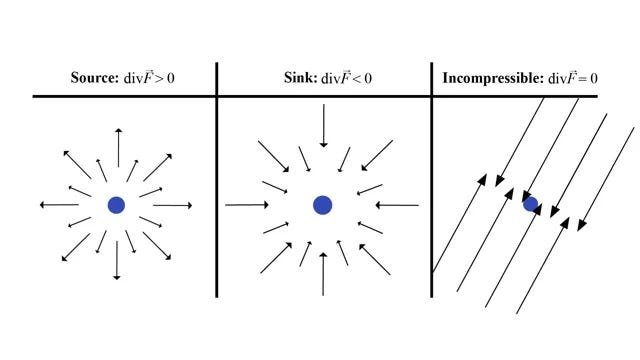
\includegraphics[width=0.5\linewidth]{images/div.jpg}
\end{center}

Geométricamente, si colocas una pequeña esfera o círculo alrededor de un punto,
y el flujo total que sale es mayor que el que entra, la divergencia es
positiva; si entra más de lo que sale, es negativa. La divergencia se calcula
como una combinación de derivadas parciales que describe cómo cambian las
componentes del campo en cada dirección. Así, la divergencia condensa en un
número local la idea de densidad de flujo saliente desde un punto del campo.\\

\begin{observación}
Sea el vector $\vec{u} = (u_1, u_2) \neq (0,0)$, entonces tenemos dos vectores ortogonales a $\vec{u}$ que son $\vec{v} = (u_2, -u_1)$ y $\vec{w} = (-u_2, u_1)$, y que se obtienen rotando $\vec{u}$ 90 grados en sentido horario y antihorario respectivamente.
\end{observación}

\begin{definición} [Vector Normal Unitario Exterior]
Sea $C \subset \mathbb{R}^2$ curva de Jordan regular a trozos en $D = Int(C)$. Sea $\gamma : [a,b] \to \mathbb{R}^2$ una parametrización regular a trozos de $C$ que induce la orientación positiva $C^+$. Para cada $t_0 \in [a,b]$, excepto una cantidad finita de ellos, consideramos el vector tangente a $\gamma$ en $\gamma(t_0)$:
$$\gamma'(t_0) = (\gamma_1'(t_0), \gamma_2'(t_0))$$
Se define entonces el vector normal unitario exterior a $C$ en $\gamma(t_0)$ como:
$$\vec{n}(\gamma(t_0)) = \left(\frac{\gamma_2'(t_0)}{\lVert \gamma'(t_0) \rVert}, -\frac{\gamma_1'(t_0)}{\lVert \gamma'(t_0) \rVert}\right)$$
\end{definición}

El vector normal unitario exterior a una curva cerrada en el plano representa
la dirección que apunta hacia fuera del dominio $D$ delimitado por la curva, y
es perpendicular al vector tangente en cada punto regular. Cuando una curva $C$
está orientada positivamente (es decir, recorriéndola el interior queda a la
izquierda), el exterior queda a la derecha del sentido de recorrido. Por tanto,
para obtener el vector normal exterior, se toma el vector tangente en ese punto
y se rota 90° en sentido horario, apuntando hacia fuera.\\

\begin{teorema} [Teorema de la Divergencia]
    Supongamos que tenemos $C \subset \mathbb{R}^2$ curva de Jordan regular a trozos con $D = Int(C)$ y sea $\vec{F} = (F_1, F_2) : U \to \mathbb{R}^2$ campo vectorial de clase $C^1$ definido en un abierto $U \supset \overline{D} = D \cup C$. Entonces:
    $$\int_{D} div(\vec{F}) = \int_{C^+} \langle \vec{F}, \vec{n} \rangle$$
    donde $\vec{n}$ es el vector normal unitario exterior a $C^+$.
\end{teorema}

\begin{proof}
    Consideramos el campo vectorial $\vec{G} = (-F_2, F_1) = (P,Q)$ y aplicamos el Teorema de Green:
    \[\int_{D} \left(\frac{\partial Q}{\partial x} - \frac{\partial P}{\partial y}\right) dx dy = \int_{C^+} Pdx + Qdy\]
    \begin{itemize}
        \item \[\int_{D} \left(\frac{\partial Q}{\partial x} - \frac{\partial P}{\partial y}\right) dx dy = \int_{D} \left(\frac{\partial F_1}{\partial x} + \frac{\partial F_2}{\partial y}\right) dx dy = \int_{D} div(\vec{F}) dx d\]
        \item \[\int_{C^+} \underbrace{\langle \vec{F}, \vec{n} \rangle}_{\text{campo escalar}} = \int_{t=a}^{t=b} \langle \vec{F}(\gamma(t)), \vec{n}(\gamma(t)) \rangle \lVert \gamma'(t) \rVert dt = \int_{t=a}^{t=b} \langle (F_1(\gamma(t)), F_2(\gamma(t))), (\gamma_2'(t), -\gamma_1'(t)) \rangle dt\]
              \[ = \int_{t=a}^{t=b} -F_2(\gamma(t))\gamma_1'(t) + F_1(\gamma(t))\gamma_2'(t) dt = \int_{C^+} Pdx + Qdy\]
    \end{itemize}
\end{proof}

Lo que nos viene a decir el teorema de la divergencia es que la cantidad total
de “campo” que se genera o se pierde dentro de una región (\(D\)) es
exactamente igual al flujo neto que atraviesa su frontera (\(C\)), medido
mediante el producto escalar del campo con el vector normal exterior. Este
resultado permite traducir una propiedad local del campo —la divergencia, que
mide en cada punto si el campo actúa como fuente o sumidero— en una propiedad
global, como el flujo total que atraviesa el borde.

En términos más concretos, el lado izquierdo de la igualdad, \( \int_D
\text{div}(\vec{F}) \), cuantifica cuánto se "crea" o "destruye" del campo
dentro del área: es una suma punto a punto de los nacimientos o desapariciones
del flujo. Por su parte, el lado derecho, \( \int_{C^+} \langle \vec{F},
\vec{n} \rangle \), mide directamente cuánto del campo está atravesando la
frontera hacia el exterior. Así, si dentro de la región hay fuentes, el campo
tiende a salir; si hay sumideros, tiende a entrar. Este teorema no solo tiene
un profundo contenido conceptual —relacionando lo interno con lo externo, lo
local con lo global—, sino que también es una herramienta práctica: convierte
una integral doble sobre una región (a menudo más complicada) en una integral
de línea a lo largo de su frontera (más manejable si se conoce el campo sobre
ella).
